\documentclass{article}
\RequirePackage[a4paper,top=2cm,left=.5cm,right=.5cm,bottom=2cm]{geometry}

\usepackage{pdfpages}
\usepackage{fp}% http://ctan.org/pkg/calc
\usepackage{tikz}
\usepackage{caption}
\usepackage{floatrow}
\usepackage{makecell}
\usepackage{lscape}
\setlength{\abovecaptionskip}{15pt plus 3pt minus 2pt} 

\pagenumbering{gobble}

\begin{document}

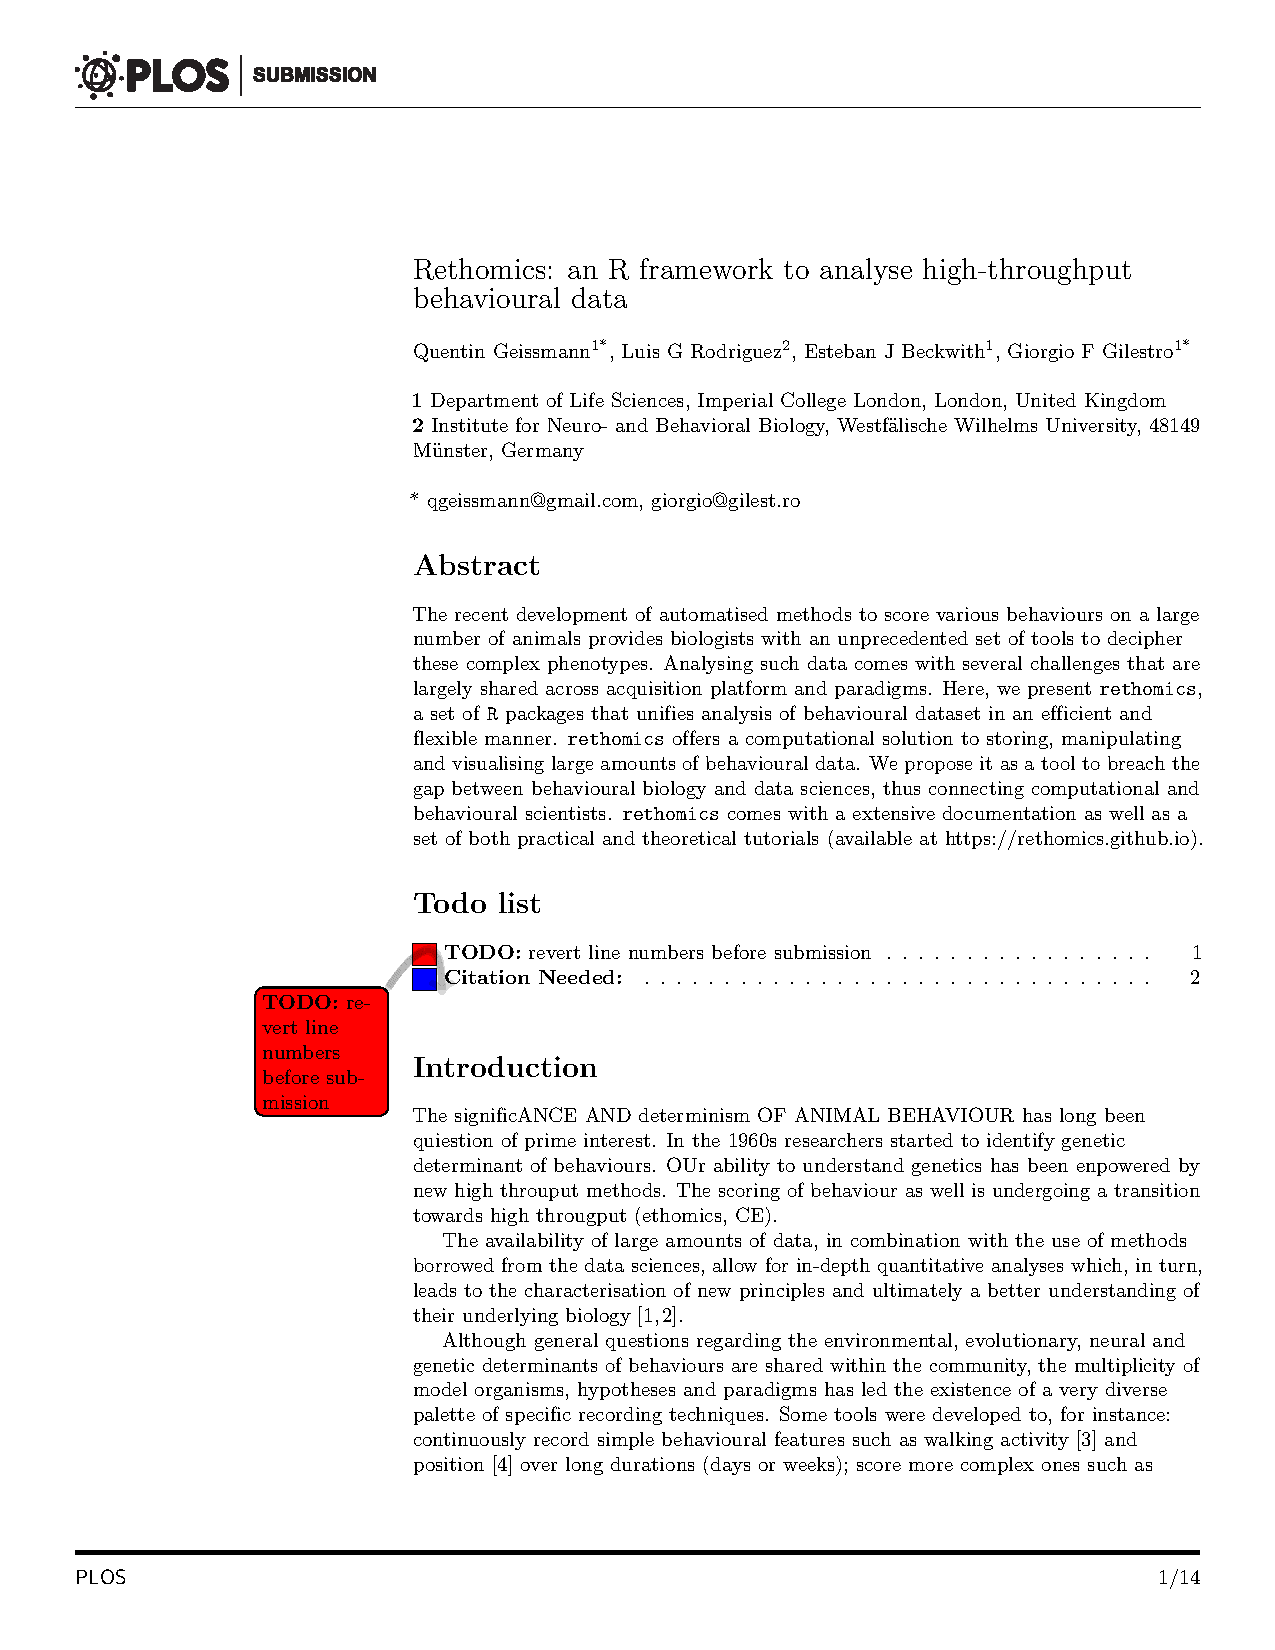
\includepdf[pages=1-]{manuscript.pdf}

\foreach \x in {1,2,3,4,5,6}
{ 	\begin{figure}[p]
		\centering  
    \begin{minipage}[c][\textheight]{\textwidth}
		\includegraphics[width=.90\textwidth, page=\x]{all-figures.pdf}
		\caption*{\LARGE{Geissmann et al. 2018, Fig \x}}
  \end{minipage}
	\end{figure}
  \clearpage	
}	

\begin{figure}[p]
	\centering  
	\begin{minipage}[c][\textheight]{\textwidth}
			\centering  
%		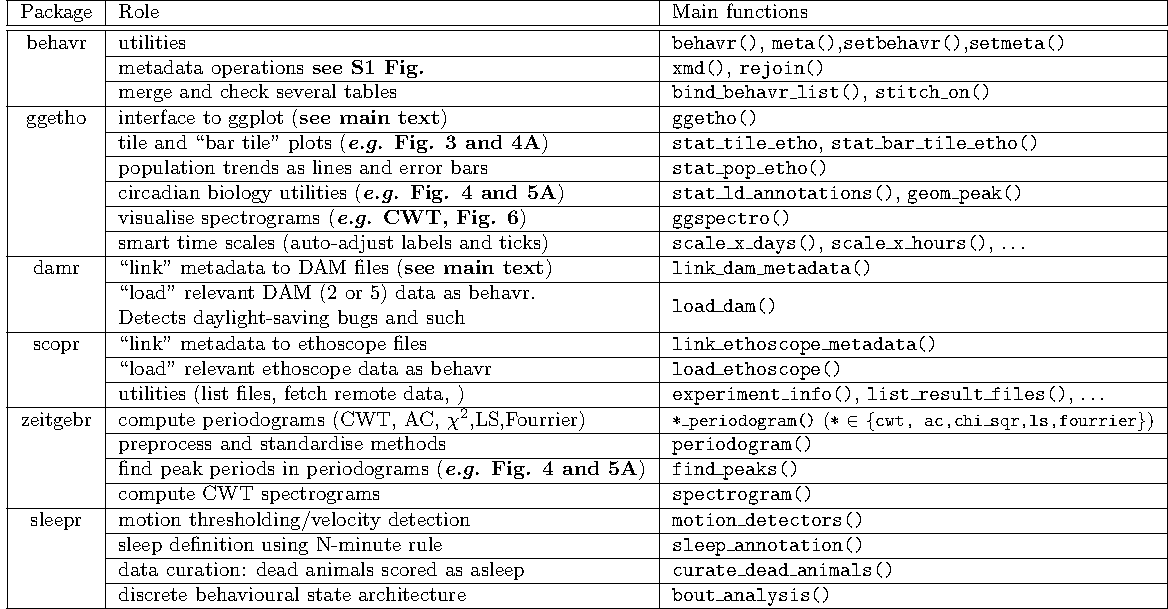
\includegraphics[width=.90\textwidth,angle=90]{functionalities_table.pdf}
		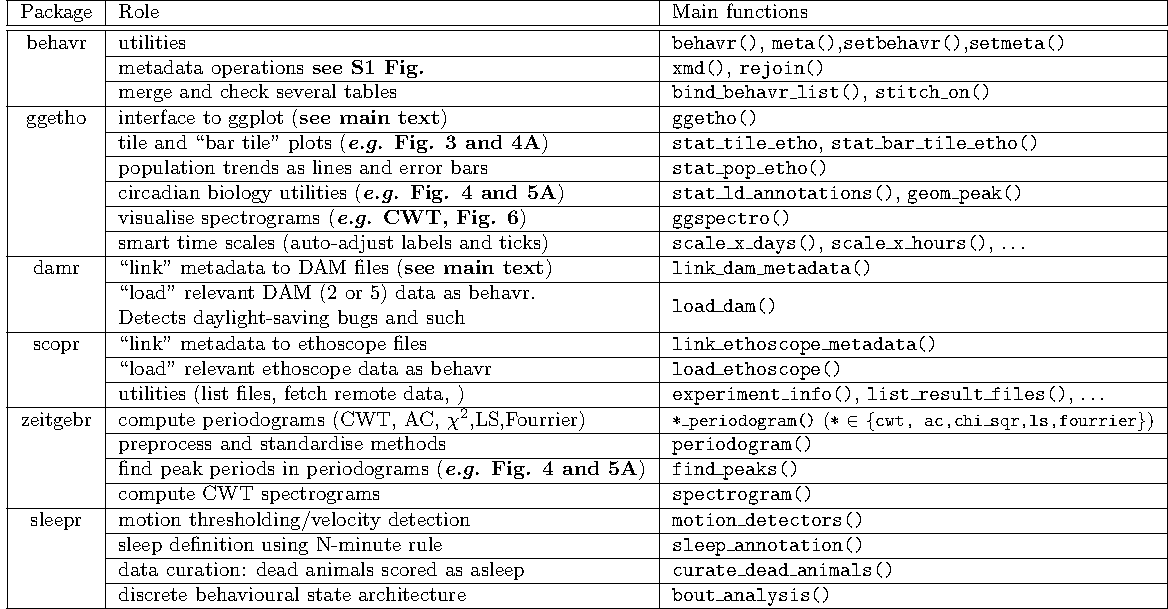
\includegraphics[width=.90\textwidth]{functionalities_table.pdf}
		\caption*{\LARGE{Geissmann et al. 2018, Table S1}}
		\end{minipage}
	\end{figure}
\clearpage	


\foreach \x in {7, 8}
{ 	
\FPeval{\result}{clip(\x-6)}
\begin{figure}[p]
		\centering  
    \begin{minipage}[c][\textheight]{\textwidth}
		\includegraphics[width=.90\textwidth, page=\x]{all-figures.pdf}
		\caption*{\LARGE{Geissmann et al. 2018, Fig S\result}}
  \end{minipage}
	\end{figure}
  \clearpage	
}		

\end{document}
